\documentclass[tikz, border=20pt]{standalone}
\usepackage{tikz}
\usetikzlibrary{arrows.meta}

\tikzset{
  pics/features/.style  args={#1/#2/#3}{% #1=depth, #2=height, #3=width
    code = {
      \coordinate (-center-out) at (#1/2, 0, 0);
      \coordinate (-center-in) at (-#1/2, 0, 0);
  \draw (-#1/2, -#2/2, #3/2) -- (#1/2, -#2/2, #3/2) -- (#1/2, #2/2, #3/2) -- (-#1/2, #2/2, #3/2) -- (-#1/2, -#2/2, #3/2);
  \draw (#1/2, -#2/2, #3/2) -- (#1/2, -#2/2, -#3/2) -- (#1/2, #2/2, -#3/2) -- (#1/2, #2/2, #3/2);
  \draw (#1/2, #2/2, -#3/2) -- (-#1/2, #2/2, -#3/2) --(-#1/2, #2/2, #3/2);
  \draw [dashed] (-#1/2, -#2/2, #3/2) -- (-#1/2, -#2/2, -#3/2) -- (#1/2, -#2/2, -#3/2);
  \draw [dashed] (-#1/2, -#2/2, -#3/2) -- (-#1/2, #2/2, -#3/2);
  \draw (0, -#2/2, #3/2) node[below]{\scriptsize 1};
  \draw (#1/2, -#2/2, 0) node[right]{\scriptsize 28};
  \draw (#1/2, 0, -#3/2) node[right]{\scriptsize 28};
  \node{\tikzpictext};
}}}

\tikzset{
  pics/dense/.style args={#1/#2/#3}{
    code = {
      \draw (-#1/2, -#2/2) -- (#1/2, -#2/2) -- (#1/2, #2/2) -- (-#1/2, #2/2) -- (-#1/2, -#2/2);
      \draw (0, -#2/2) node[below]{\scriptsize #3};
}}}

\tikzset{
  pics/conv/.style args={#1/#2}{
    code = {
      \draw [dashed] (0, -#1/2, -#2/2) -- (2, 0, 0);
      \draw [dashed] (0, -#1/2, #2/2) -- (2, 0, 0);
      \draw [dashed] (0, #1/2, #2/2) -- (2, 0, 0);
      \draw [dashed] (0, #1/2, -#2/2) -- (2, 0, 0);
      \draw (0, -#1/2, -#2/2) -- (0, -#1/2, #2/2) -- (0, #1/2, #2/2) -- (0, #1/2, -#2/2) -- (0, -#1/2, -#2/2);
      \draw (0, 0, #2/2) node[left]{\scriptsize 3};
      \draw (0, #1/2, 0) node[above]{\scriptsize 3};

    }
  }
}

\begin{document}

\tikzstyle{box} = [draw, rectangle, rounded corners, color=black!80, fill=gray!20!blue!10, minimum width=7em, minimum height=3.5em]
\tikzstyle{line>} = [-{Latex[length=2mm]}, color=black!80]
\tikzstyle{<line} = [{Latex[length=2mm]}-, color=black!80]




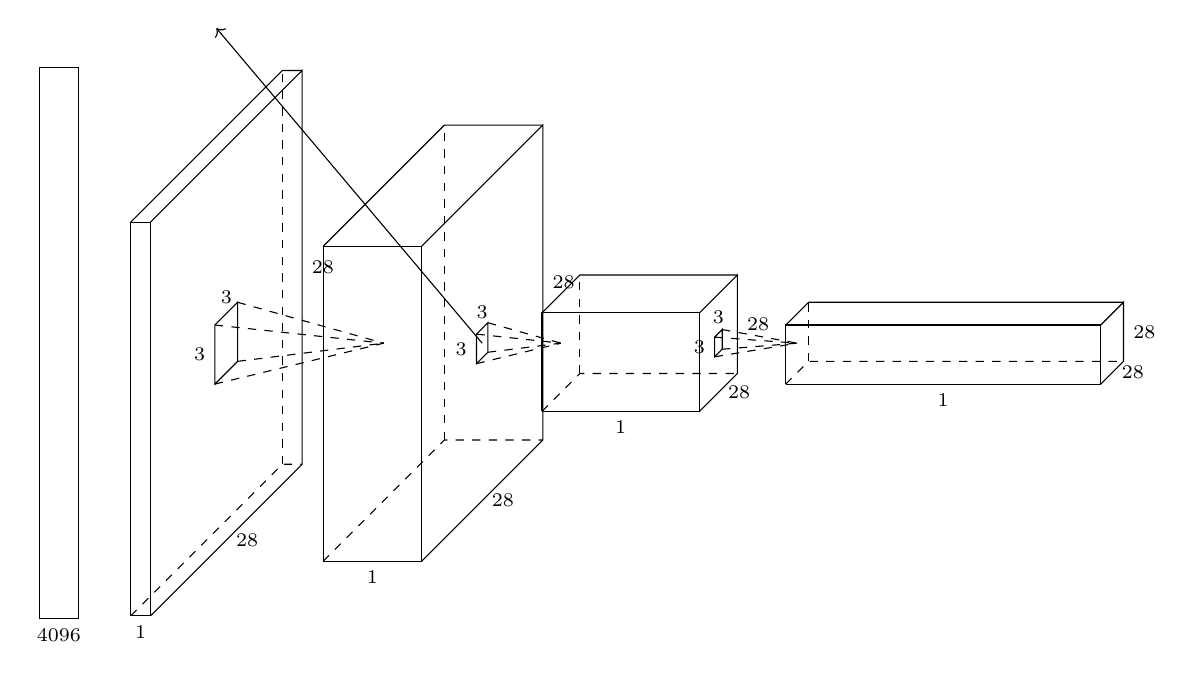
\begin{tikzpicture}
  \draw (1, 0) pic{dense={0.5/7/4096}};
  \draw (3, 0) pic{features={0.25/5/5}};
  \draw (3.125, 0) pic{conv={0.75/0.75}};
  % \draw (5.75, 0) pic[color=black]{features={1.25/4/4}};
  \pic[color=black] (one) at (5.75, 0) {features={1.25/4/4}};
  \draw [->] (one-center-out) -- (3, 4);
  \draw (6.375, 0) pic[scale=0.5]{conv={0.75/0.75}};
  \draw (8.375, 0) pic[color=black]{features={2/1.25/1.25}};
  \draw (9.375, 0) pic[scale=0.5]{conv={0.5/0.5}};
  \draw (12.375, 0) pic[color=black]{features={4/0.75/0.75}};

\end{tikzpicture}

\end{document}
